\documentclass{beamer}
\mode<presentation> {
% The Beamer class comes with a number of default slide themes
% which change the colors and layouts of slides. Below this is a list
% of all the themes, uncomment each in turn to see what they look like.

%\usetheme{default}
%\usetheme{AnnArbor}
%\usetheme{Antibes}
%\usetheme{Bergen}
%\usetheme{Berkeley}
%\usetheme{Berlin}
%\usetheme{Boadilla}
%\usetheme{CambridgeUS}
%\usetheme{Copenhagen}
%\usetheme{Darmstadt}
%\usetheme{Dresden}
%\usetheme{Frankfurt}
%\usetheme{Goettingen}
%\usetheme{Hannover}
%\usetheme{Ilmenau}
%\usetheme{JuanLesPins}
%\usetheme{Luebeck}
\usetheme{Madrid}
%\usetheme{Malmoe}
%\usetheme{Marburg}
%\usetheme{Montpellier}
%\usetheme{PaloAlto}
%\usetheme{Pittsburgh}
%\usetheme{Rochester}
%\usetheme{Singapore}
%\usetheme{Szeged}
%\usetheme{Warsaw}
\usepackage{fancyhdr}
\usepackage{animate}
\usepackage{caption}
\usepackage{subcaption}

% As well as themes, the Beamer class has a number of color themes
% for any slide theme. Uncomment each of these in turn to see how it
% changes the colors of your current slide theme.

%\usecolortheme{albatross}
%\usecolortheme{beaver}
%\usecolortheme{beetle}
%\usecolortheme{crane}
%\usecolortheme{dolphin}
%\usecolortheme{dove}
%\usecolortheme{fly}
%\usecolortheme{lily}
%\usecolortheme{orchid}
%\usecolortheme{rose}
%\usecolortheme{seagull}
%\usecolortheme{seahorse}
%\usecolortheme{whale}
%\usecolortheme{wolverine}

%\setbeamertemplate{footline} % To remove the footer line in all slides uncomment this line
\setbeamertemplate{footline}[page number] % To replace the footer line in all slides with a simple slide count uncomment this line

\setbeamertemplate{navigation symbols}{} % To remove the navigation symbols from the bottom of all slides uncomment this line
}

\usepackage{graphicx} % Allows including images
\usepackage{booktabs} % Allows the use of \toprule, \midrule and \bottomrule in tables
\usepackage{multirow} % Allows use of multirow
%\usepackage {tikz}
\usepackage{tkz-graph}
\GraphInit[vstyle = Shade]
\tikzset{
  LabelStyle/.style = { rectangle, rounded corners, draw,
                        minimum width = 2em, fill = yellow!50,
                        text = red, font = \bfseries },
  VertexStyle/.append style = { inner sep=5pt,
                                font = \normalsize\bfseries},
  EdgeStyle/.append style = {->, bend left} }
\usetikzlibrary {positioning}
%\usepackage {xcolor}
\definecolor {processblue}{cmyk}{0.96,0,0,0}
%----------------------------------------------------------------------------------------
%	TITLE PAGE
%----------------------------------------------------------------------------------------

\title[Short title]{Particle Filter based SLAM} % The short title appears at the bottom of every slide, the full title is only on the title page

\author{Aswin P Ajayan} % Your name
\institute[Indian Institute of Technology, Bombay] % Your institution as it will appear on the bottom of every slide, may be shorthand to save space
{
Indian Institute of Technology, Bombay\\ % Your institution for the title page
\medskip
}
\date{Jun 30, 2020} % Date, can be changed to a custom date

\begin{document}

\begin{frame}
\titlepage % Print the title page as the first slide
\end{frame}

\begin{frame}
\frametitle{Overview} % Table of contents slide, comment this block out to remove it
\tableofcontents % Throughout your presentation, if you choose to use \section{} and \subsection{} commands, these will automatically be printed on this slide as an overview of your presentation
\end{frame}

%----------------------------------------------------------------------------------------
%	PRESENTATION SLIDES
%----------------------------------------------------------------------------------------

%------------------------------------------------

\section{What is SLAM}
\begin{frame}{What is SLAM}
    \begin{itemize}
    \item Computing robot's poses and map environment simultaneously \\
    \item Localisation : estimating robots location\\ 
    \item Mapping      : building a MAP\\
    \item Given
    \begin{itemize}
        \item $u_{1:T} = \{u_1,u_2,u_3....u_T\}$, the control inputs
        \item $z_{1:T} = \{z_1,z_2,z_3,...,z_T\}$, observations

    \end{itemize}
\item Wanted
    \begin{itemize}
    \item $m$, map of the environment
    \item $x_{0:T} = \{x_0,x_1,x_2,...,x_T\}$ , robot location
    \item $p(x_{0:T},m | u_{0:T},z_{1:T})$, the SLAM posterior
        \end{itemize}
\end{itemize}


\end{frame}


\section{Objective}
\begin{frame}{Objective}
    \begin{itemize}
        \item To review the literature available on SLAM. To get acquainted with various techniques available for SLAM and examine some of them in depth. Simulation in reallife constraints using ROS.\\
            Types of SLAM techniques explored includes
        \item \textbf{Kalman Filter based approaches}
            \begin{itemize}
                \item Extended Kalman Filter
                \item Unscented Kalman Filter
                \item Extended Information Filter
            \end{itemize}
            \item \textbf{Particle Filter based approaches}
                \begin{itemize}
                    \item Fast SLAM -Rao Blackwellised Particle Filter
                \end{itemize}
                \begin{figure}[H]
        \centering
        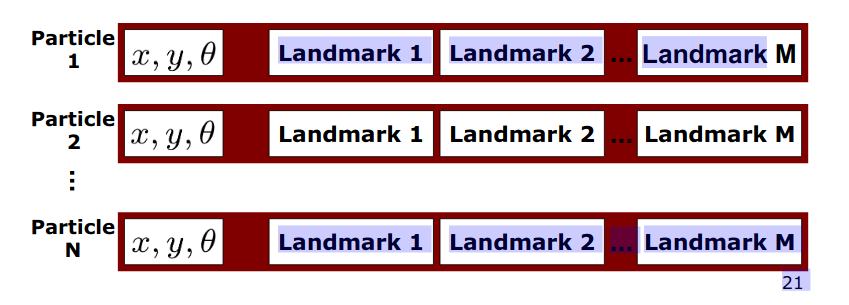
\includegraphics[width = 100mm]{RBPF_SLAM.png}$^{1}$
        \end{figure}
    \end{itemize}
\vfill
\tiny Image Source:
\newline \tiny{$^{1}$}https://www.opli.net/opli\_magazine/imaging/2017/sierra-olympic-introduces-world-first-true-hd-thermal-camera-jan-news/
\newline \tiny{$^{2}$}https://in.element14.com/terasic-technologies/p0082/e22f17c6n-DEO-nano-dev-kit/dp/2076463
\newline \tiny{$^{3}$}http://www.123-cctv.com/CCTV-Monitors/7-inch-Security-LCD-Monitor-with-VGA.html
\end{frame}



\begin{frame}{Components}
    \begin{itemize}
        \item Infrared Camera - DLC384 Long Wave Infrared Focal Plane Array 384X288 25um Uncooled Microbolometer.
        \item FPGA - DEO-Nano Development Board.
        \item Software - Quartus Prime Lite Edition.
        \item Programming Language - Very High Speed Integrated Circuit Hardware Description Language (VHDL).
    \end{itemize}
\end{frame}


\section{Block Diagram of Camera Driver}
\begin{frame}{Block Diagram of Camera Driver}
    \begin{figure}[H]
        \centering
        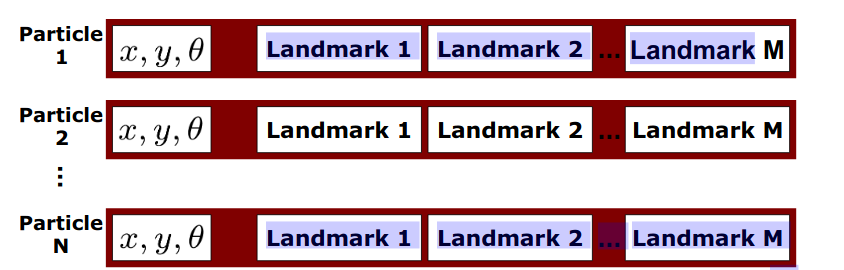
\includegraphics[width=\textwidth]{RBPF_particles.png}$^{2}$
        \end{figure}
\end{frame}


\begin{frame}{Components of Camera Driver}
    \begin{itemize}
        \item DLC384 Sensor.
        \item Camera Driver - 
        \begin{itemize}
            \item PLL and DLC384 reading FSM.
            \item Address Cal and Dual Port RAM.
            \item DLC384 Controller.
            \item ADC - Analog to Digital Converter.
        \end{itemize}
    \end{itemize}
\end{frame}


\section{DLC384 Sensor}
\begin{frame}{DLC384 Sensor}
    \begin{itemize}
        \item This is a long Wave Infrared Focal Plane Array(IRFPA), 384X288, 25 um Uncooled Microbolometer. Spectral range of 8um~14um.
        \item DLC384 works in rolling shutter mode, meaning integration of one row at a time and simultaneous reading of previous row.
        \item We will see what is IRFPA and ROIC to better understand the device like DLC384, in general.
        \item \textbf{IRFPA} - Is an infrared(IR) image sensing device consisting of an array of IR sensing pixels placed at the focal point of a lense. This convert IR radiations to electrical signals. These IR sensing pixels can be a bolometer(in case of DLC384) which changes resistance if IR radiation is incident on it. IR detector are cooled to improve the signal to noise ratio (S/N) and to keep the temperature of the detector at a constant point in DLC384 thermoelectric cooling is used.
        \item \textbf{ROIC} - It is a silicon chip with circuit that integrate, sample and holds, amplify and multiplex the week detector current. % This is Interface b/w IRFPA and Camera Driver.
        \begin{figure}
            \hfil
            \hfil
            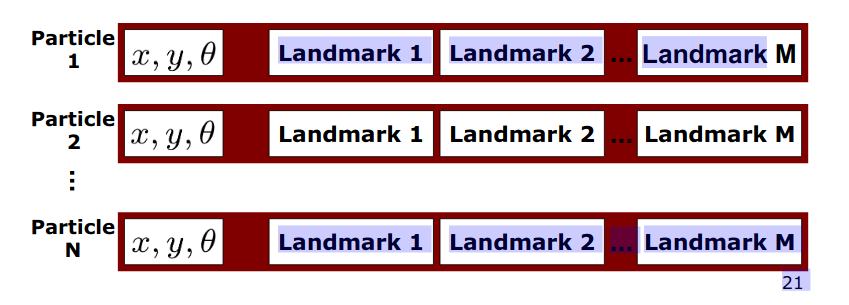
\includegraphics[width = 20mm]{RBPF_SLAM.png}
        \end{figure}
    \end{itemize}
\end{frame}


\begin{frame}{DLC384 Sensor Pin Diagram}
   \begin{figure}
            \centering
            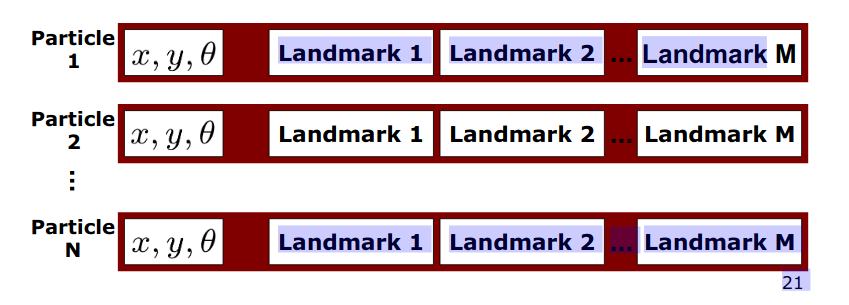
\includegraphics[width=100mm]{RBPF_SLAM.png}$^{3}$
    \end{figure}
\vfill
\tiny{$^{4}$} Source: DLC384 User Manual
\end{frame}


\begin{frame}{Example circuit for signal pathway from one pixel to the output}
   \begin{figure}
            \centering
            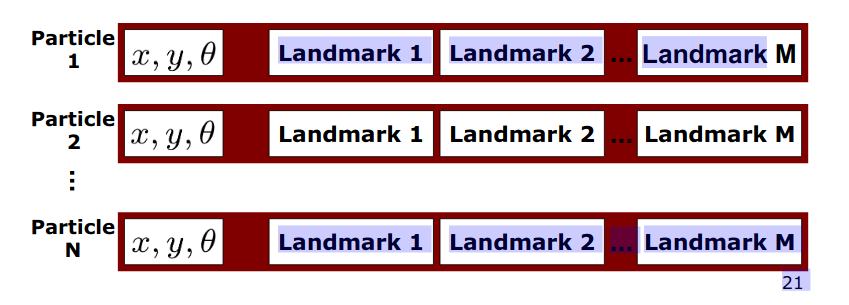
\includegraphics[width= 100mm]{RBPF_SLAM.png}$^{4}$
    \end{figure}
    \begin{figure}
            % \hfil
            \hfill
            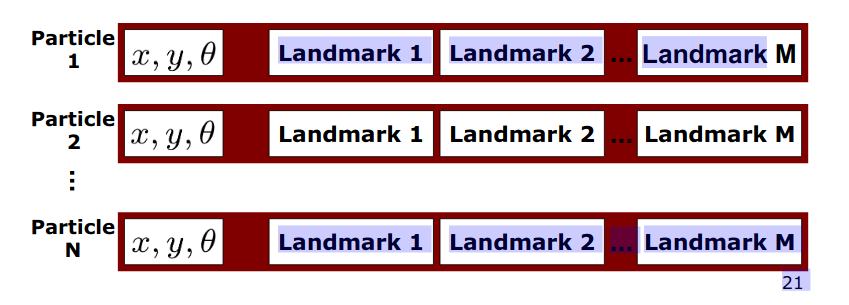
\includegraphics[width = 50mm]{RBPF_SLAM.png}
    \end{figure}
\vfill
\tiny{$^{5}$} Source: A Design of Readout Circuit for 384x288 Uncooled Microbolometer Infrared Focal Plane Array - 2012 IEEE 11th International Conference on Solid-State and Integrated Circuit Technology
\end{frame}


\begin{frame}{Working of IRFPA and ROIC using example circuit}
    \begin{itemize}
        \item For each N{$^{th}$}-column there will be a blind pixel, a Integrator and sample and hold circuit, a output buffer (in rolling shutter mode). Output buffers are multiplex on “Vout” pin which is read by camera driver after digitization of its analog value.
        \item The induced small current because of change in resistance of Active Pixel by the IR radiation is integrated. This integrated voltage is stored in capacitor “Cint”. Usually this integration happen till the “INT” signal is high, coming from camera driver.
        \item Simultaneously previous row pixels value which is hold in capacitor “Csh” is read. Usually the reading of all the pixels of a row by camera driver happen till the “VOUT\_EN” signal is high. This signal is set/reset by ROIC.
        \item After integration of all the pixels of a row and reading of all the pixels of previous row, “VOUT\_EN” and “INT” are low, and the integrated voltage from “Cint” is sampled and hold to “Csh”.
    \end{itemize}
\end{frame}


\begin{frame}{Working of IRFPA and ROIC using example circuit (continue)}
    \begin{itemize}
        \item A control unit is part of the ROIC which multiplex row and column data to “VOUT”.
        \item Integrator, sample and hold (S/H) circuit can be same for a column (in rolling shutter mode)  or a part of unit cell (in Global shutter mode).
        \item While reading the voltage from “Csh”, next row (in rolling shutter mode)  or next frame (in Global shutter mode) is integrated on "Cint".
    \end{itemize}
\end{frame}


\begin{frame}{Block diagram of IRFPA and ROIC for Rolling and Global shutter Mode }
   \begin{figure}
        \centering
        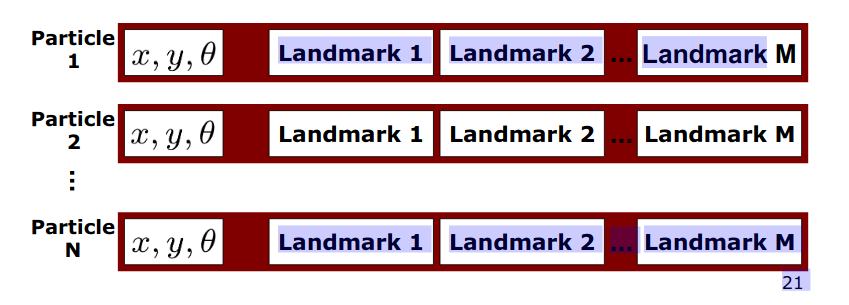
\includegraphics[width= 100mm]{RBPF_SLAM.png}$^{5}$
    \end{figure}
    \vfill
    \tiny Source:
    \newline \tiny{$^{5}$}A Design of Readout Circuit for 384x288 Uncooled Microbolometer Infrared Focal Plane Array - 2012 IEEE 11th International Conference on Solid-State and Integrated Circuit Technology
    \newline \tiny{$^{6}$}Large dynamic range Readout Integrated Circuit for Infrared Detectors -2019 32nd International Conference on VLSI Design and 2019 18th International Conference on Embedded Systems (VLSID)
\end{frame}


\begin{frame}{Clock Diagram of DLC384}
    \begin{figure}
        \centering
        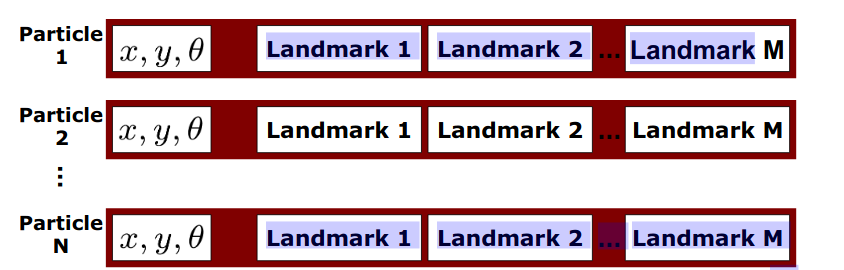
\includegraphics[width=\textwidth]{RBPF_particles.png}$^{6}$
    \end{figure}
    \vfill
    \tiny{$^{4}$} Source: DLC384 user manual
\end{frame}


\begin{frame}{Explanation of DLC384 Clock Diagram}
    \begin{itemize}
        \item Input to DLC384 from camera driver(which is implemented on FPGA) - “MCLK”, “INT”, “RST”.
        \item Output from DLC384 to camera driver- “VOUT-EN”, “FR”, “VOUT”(VOUT is a analog signal which is connected to camera driver  via n-bit ADC.
        \item DLC384 works in rolling shutter mode, meaning integration of one row at a time and simultaneous reading of previous row.
        \item After “RST” is asserted from high to low, camera driver should set “INT” signal to high for maximum of  384 cycles. “RST” reset the Readout IC operation of sensor by forcing the integration of the signal on the first row.
        \item After “INT” signal is asserted low (by camera driver), DLC384 will set “VOUT\_EN” and “FR” to high after exactly 18.5 cycles.
        \item “FR” trigger to high mark the start of the first row of a frame.
    \end{itemize}
\end{frame}


\begin{frame}{Explanation of DLC384 Clock Diagram (continue)}
    \begin{itemize}

        \item From this point onwards pixel values of 1st row is available on “VOUT”, and on every rising edge of clock next pixel value is loaded on “VOUT”. Simultaneously “INT” should be asserted high by camera driver for maximum of 384 cycles so that integration of the signal on the next row can be done.
        \item Once all the pixels of a row are read (after 384 cycles), “VOUT\_EN” will assert to 0 and after 18.5 cycles from “INT” falling edge it will assert to high so that next rows pixels can be read.
    \end{itemize}
\end{frame}


\section{Camera Driver}
\begin{frame}{Camera Driver}
    Camera Driver have following Components -
    \begin{itemize}
        \item \textbf{Phase Locked Loop (PLL)-} Generated using the megafunction of quartus prime, generating 6.25 MHz so that 50 frames per second can be read from DLC384. It’s input is from a 50 MHz onboard oscillator.
        \item \textbf{DLC384 reading FSM-} This on sensing inputs from IR sensor (VOUT\_EN, FR) and Resetn from onboard switch, produces signals(INT, H\_Counter, V\_Counter) to read pixels value and store it to the “Dual Port RAM”.
        \item \textbf{Address Cal-} Using H\_Counter, V\_Counter this module calculate the index/address (= count\_V * number of column + count\_H) of the pixel. Output of this module is connected to Dual Port RAM read address line.
        \item \textbf{Dual Port RAM-} Generated using the megafunction of quartus prime. 8 bit word length and 2\^16 bits addressable. Simultaneously read and write operation can be performed, can be further interfaced with VGA Port 
        \item \textbf{DLC384 Controller-} Configures the DLC384 Sensor
    \end{itemize}
\end{frame}


\begin{frame}{RTL of Camera Driver}
    \begin{figure}
        \centering
        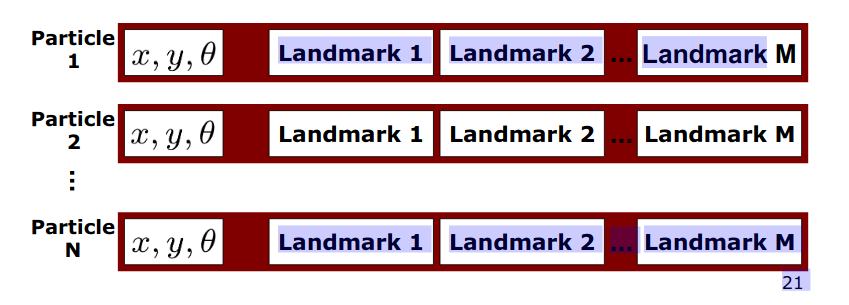
\includegraphics[width=\textwidth]{RBPF_SLAM.png}$^{7}$
    \end{figure}
\end{frame}


% \begin{frame}{DLC384 Reading FSM Diagram}
%      \begin{figure}
%         \includegraphics[width = 100mm]{DLC384-reading-FSM.png}$^{8}$
%     \end{figure}   
% \end{frame}


\begin{frame}{Analysis of DLC384 Reading FSM Diagram and clock diagram from data sheet}
     \begin{figure}
     \centering
        \begin{subfigure}[b]{0.4\textwidth}
        % \centering
        \hspace*{-10mm}
        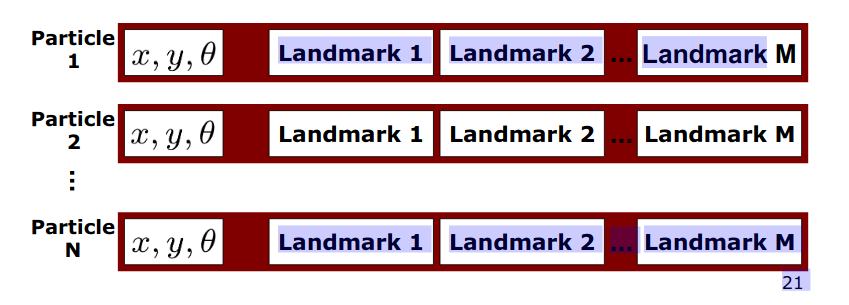
\includegraphics[height = 60mm,width = 60mm]{RBPF_SLAM.png}
        \end{subfigure}
    ~
        \begin{subfigure}[b]{0.4\textwidth}
        \centering
        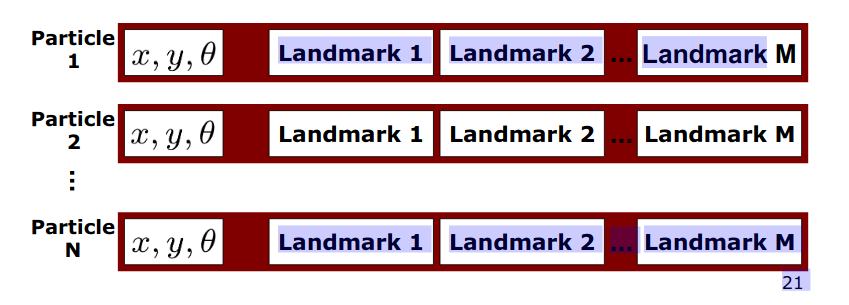
\includegraphics[height = 60mm,width = 60mm]{RBPF_SLAM.png}$^{8}$
        \end{subfigure}
    \end{figure}   
\end{frame}


\begin{frame}{DLC384 Reading FSM}
     \begin{itemize}
         \item DLC384 Reading FSM is a finite state machine having 4 states, a) State\_Reset; b) State\_INT; c) State\_EN; d) State\_Read.
         \item States (c) and (d) are two main states, in which FSM toggle’s maximum amount of time.
         \item In state (C) FSM waits for “VOUT\_EN” signal from DLC384 which is expected to arrive after 18.5 cycles from “INT” falling edge.
         \item In State (d) “INT” signal is high( for 384 cycles) so that integration of next row pixels can be done. Also since VOUT\_EN is high so simultaneously current row’s pixels value is captured at every rising edge of clock.
     \end{itemize}
\end{frame}


\begin{frame}{DLC384 Controller FSM Diagram}
    \begin{figure}
        \centering
        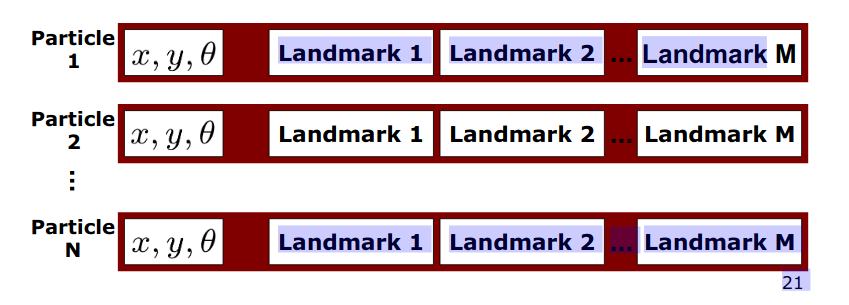
\includegraphics[width=\textwidth]{RBPF_SLAM.png}$^{9}$
    \end{figure}
\end{frame}


\begin{frame}{DLC384 Controller}
    \begin{itemize}
        \item There are two different input pins used to configure this sensor, SERIAL and SERDAT.
        \item If SERIAL = 0V then SERDAT is off and CTIA capacitance (on which integration charge accumulates) is fixed to 14 pF.
        \item If SERIAL = 5 V and SERDAT = 0V then CTIA capacitance is fixed to 18 pF or by sending some bit streams via SERDAT pin we can set different CTIA capacitance and different functions of the sensor can also be changed like(HFLIP,VFLIP).
        \item As can be seen in FSM diagram of the DLC384 controller, which transmit 51 bits from SERDAT pin if SERIAL pin is high.
        \item SERIAL pin is connected to DIP pin of FPGA board which can be turn on/off externally.
        \item Bit streams are hardcoded in FPGA which can be later controlled from DIP switches.
    \end{itemize}
\end{frame}


\section{Pin Configuration}
\begin{frame}{Pin Configuration and it's Key Number}
    \begin{table}[]
        \centering
        \resizebox{\textwidth}{!}{\begin{tabular}{|c|c|c|c|c|c|}
            \hline
            \textbf{In Port} & \textbf{Pin} & \textbf{Key} & \textbf{Out Port} & \textbf{Pin} & \textbf{Key} \\
            \hline
             resetn & j15 & Key0 & reset\_out & PIN\_A2 & GPIO\_02 \\
            \hline
            inclk & R8 & 50 MHz osc & int & PIN\_A3 & GPIO\_03 \\
            \hline
            vout\_en & PIN\_D3 & GPIO\_00 & clock\_6.25 & PIN\_B3 & GPIO\_04 \\
            \hline
            fr & PIN\_C3 & GPIO\_01 & pll\_locked & PIN\_A15 & LED0 \\
            \hline
              \multirow{2}{*}{Vout\_ADC} & PIN\_A4,B5,A5, & GPIO\_06 & serial\_out & PIN\_B4 & GPIO\_05 \\
              \cline{4-6} 
             & D5,B6,A6,B7,D6 & to GPIO\_013 & serdat & PIN\_A4 & GPIO\_06 \\
            \hline
            \end{tabular}}
        \caption{1}
    \end{table}
\end{frame}


\section{FPGA Resources Used}
\begin{frame}{Resources Used}
    \begin{table}[]
        \centering
        \resizebox{\textwidth}{!}{\begin{tabular}{|c|c|}
            \hline
            \textbf{Resource Name} & \textbf{Number/\% used} \\
            \hline
             Total Logic Elements & 153/22320 (less than 1\%)\\
            \hline
            Total Registers & 44 \\
            \hline
            Total Memory Bits & 524288/608256 (86\%) \\
            \hline
            Total PLLs & 1/4 (25\%) \\
            \hline
            
            \end{tabular}}
        \caption{2}
    \end{table}
\end{frame}



\section{Simulation Results}
\begin{frame}{Simulation Results Part-1: Control Signal analysis}
    \begin{figure}
        \centering
        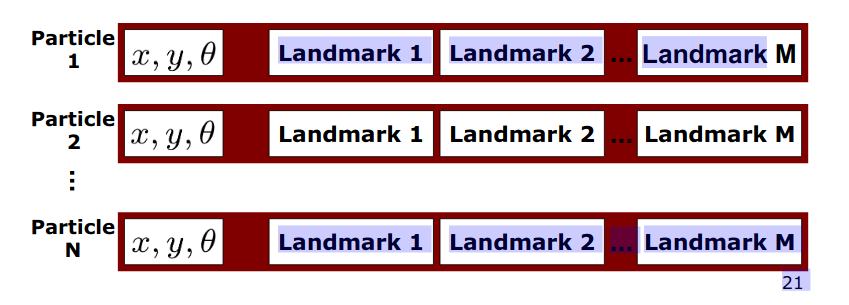
\includegraphics[width=\textwidth]{RBPF_SLAM.png}$^{10}$
    \end{figure}
\end{frame}


\begin{frame}{Simulation Results Part-1: Control Signal analysis}
    \begin{itemize}
        \item To compare the simulated timing pulses of control signals with data sheet of DLC384 it is assumed that in a frame -
            \begin{itemize}
                \item Number of columns are 5, in place of 384.
                \item Number of Rows are 3, in place of 288.
                \item Number of cycles after which the next row is read (VOUT\_EN is asserted to ‘1’ after INT is asserted to ‘0”) is 2.5 in place of 18.5.
            \end{itemize}
        \item Simulation timing pulses of control signals (figure-10) and Clock Diagram of DLC384 (figure-6) overlaps.
        \item we can calculate the pulse duration by looking at following counter values (In Figure-10).
            \begin{itemize}
                \item For 2.5 cycle(for sensor it is 18.5), for which “VOUT\_EN” is low, look for “q\_18\_cycle”.
                \item For 5 cycle(for sensor it is 384), for which “VOUT\_EN” and “INT” are high, look for “s\_h\_counter”.
                \item For current “s\_v\_count” to be seen.
            \end{itemize}
    \end{itemize}
\end{frame}


\begin{frame}{Simulation Results Part-1: Control Signal analysis (continue)}
    \begin{itemize}
        \item Using “s\_v\_count” and “s\_h\_count” values current pixel location/index can be calculated.
        \item For reset, look for “s\_reset\_out”.
        \item 6.25 MHz clock is “s\_clock\_6\_out”.
        \item Signal “fr” marks the start of a new frame, after reset is done.
        \item If "s\_serial" is high then "s\_serial\_out" is set to high and at "s\_serdat" configuration bits are sent.
    \end{itemize}
\end{frame}



\begin{frame}{Simulation Results Part-2: Working on actual images stored in a text file}
    \begin{itemize}
        \item 3 images of same pixel size is taken, considered as 3 consecutive frames of a
video.(img\_1.png, img\_2.png, img\_3.png)
        \item Using a python script, images are converted into a single vector and then saved
in a file one after another. This file will simulate the camera pixels.(Python script -
image\_to\_text.ipynb , file - img\_1\_2\_3.txt)
        \item In Quartus, a test bench is created which simulates the Camera sensor DLC384
sensor and read file “img\_1\_2\_.txt” for throwing pixels value.
        \item Sensor DLC384 gives analog value at VOUT pin, so a ADC considered b/w the
sensor and the camera driver.
        \item Once a frame is sent, testbench reads the Dual Port RAM and saves the data in
another file “output\_img.txt”.
        \item After the simulation both “img\_1\_2\_3.txt” and “out\_img.txt” files are compared
using a python script, which shows both matches perfectly.
    \end{itemize}
\end{frame}

\begin{frame}{Simulation Results Part-3: DLC384 Controller}
    \begin{itemize}
        \item DLC384 Controller simulation can be seen in figure-10, where “s\_serial\_out” and
s\_serdat” should be connected to “SERIAL” and “SERDAT” pins of the DLC384 sensor.
    \end{itemize}
\end{frame}


\section{Future Work}
\begin{frame}{Future Work}
\begin{itemize}
    \item Built an interface between Dual Port RAM(ping\_pong concept can also be introduced) and VGA port, so the video can be observed on a VGA ,monitor.
    \item DeO-Nano development board give 3.3 V as high and 0V as low, but Sensor pins works at 5V(as high) and 0V(as low) so level-shifter circuit need to be used.
\end{itemize}
\end{frame}

\section{References}
\begin{frame}{References}
\begin{thebibliography}{}
\setbeamertemplate{bibliography item}[text]
\bibitem{1} https://www.opli.net/opli\_magazine/imaging/2017/sierra-olympic-introduces-world-first-true-hd-thermal-camera-jan-news/
\bibitem{2} https://in.element14.com/terasic-technologies/p0082/e22f17c6n-DEO-nano-dev-kit/dp/2076463
\bibitem{3} http://www.123-cctv.com/CCTV-Monitors/7-inch-Security-LCD-Monitor-with-VGA.html
\bibitem{4} DLC384 User Manual
\bibitem{5} A Design of Readout Circuit for 384x288 Uncooled Microbolometer Infrared Focal Plane Array - 2012 IEEE 11th International Conference on Solid-State and Integrated Circuit
\bibitem{6} Large dynamic range Readout Integrated Circuit for Infrared Detectors -2019 32nd International Conference on VLSI Design and 2019 18th International Conference on Embedded Systems (VLSID)
\end{thebibliography}
\end{frame}


\begin{frame}
\Huge{\centerline{Thank You for your Attention}}
\end{frame}

\end{document}
